\subsection{Subpaso 1-A: Iniciar estadísticas por Opiniones del cuestionario}
	En la configuración de las estadísticas se tiene que seleccionar el 
	inciso \textbf{Opiniones del cuestionario}.
		
	\begin{figure}[hbtp]

	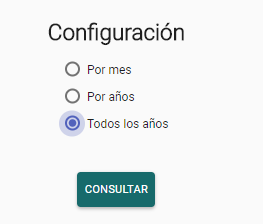
\includegraphics[scale=0.5]{images/Interfaz/IUGS15_configuracioTodos.PNG}
	\caption{Configuración por Todos los Años }
	\end{figure}
	
	
\subsection{Subpaso 1-B: Muestra de Opiniones generales}
	Se mostrará la siguiente interfaz con las siguientes opiniones generales del 
	cuestionario:
	\begin{figure}[hbtp]
		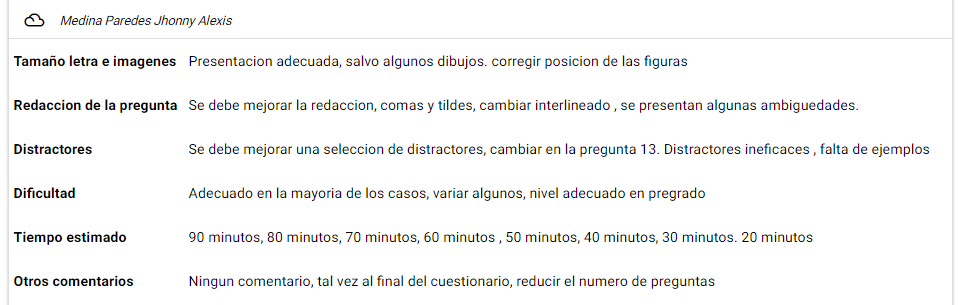
\includegraphics[scale=0.3]{images/Interfaz/IUGS15_estadisticasTodos.PNG}
		\caption{Opiniones del cuestionario por profesor}
	\end{figure}	
	Con las siguientes características
\begin{itemize}
	\item Tamaño de letra e imágenes   
	\item Redacción de la pregunta 
	\item Distractores

	\item Dificultad
	\item Tiempo Estimado
	\item Otros comentarios 
	
\end{itemize}